% !TEX TS-program = pdflatex
% !TEX encoding = UTF-8 Unicode
\documentclass[border=0mm]{standalone}
% packages
\usepackage{tikz}
\usetikzlibrary{patterns}
\usepackage{amsmath,amssymb}
\usepackage{bm}
\usepackage{pgfplots}
\pgfplotsset{compat=1.15}
% start document
\begin{document}
% generated by ROOT (CERN)
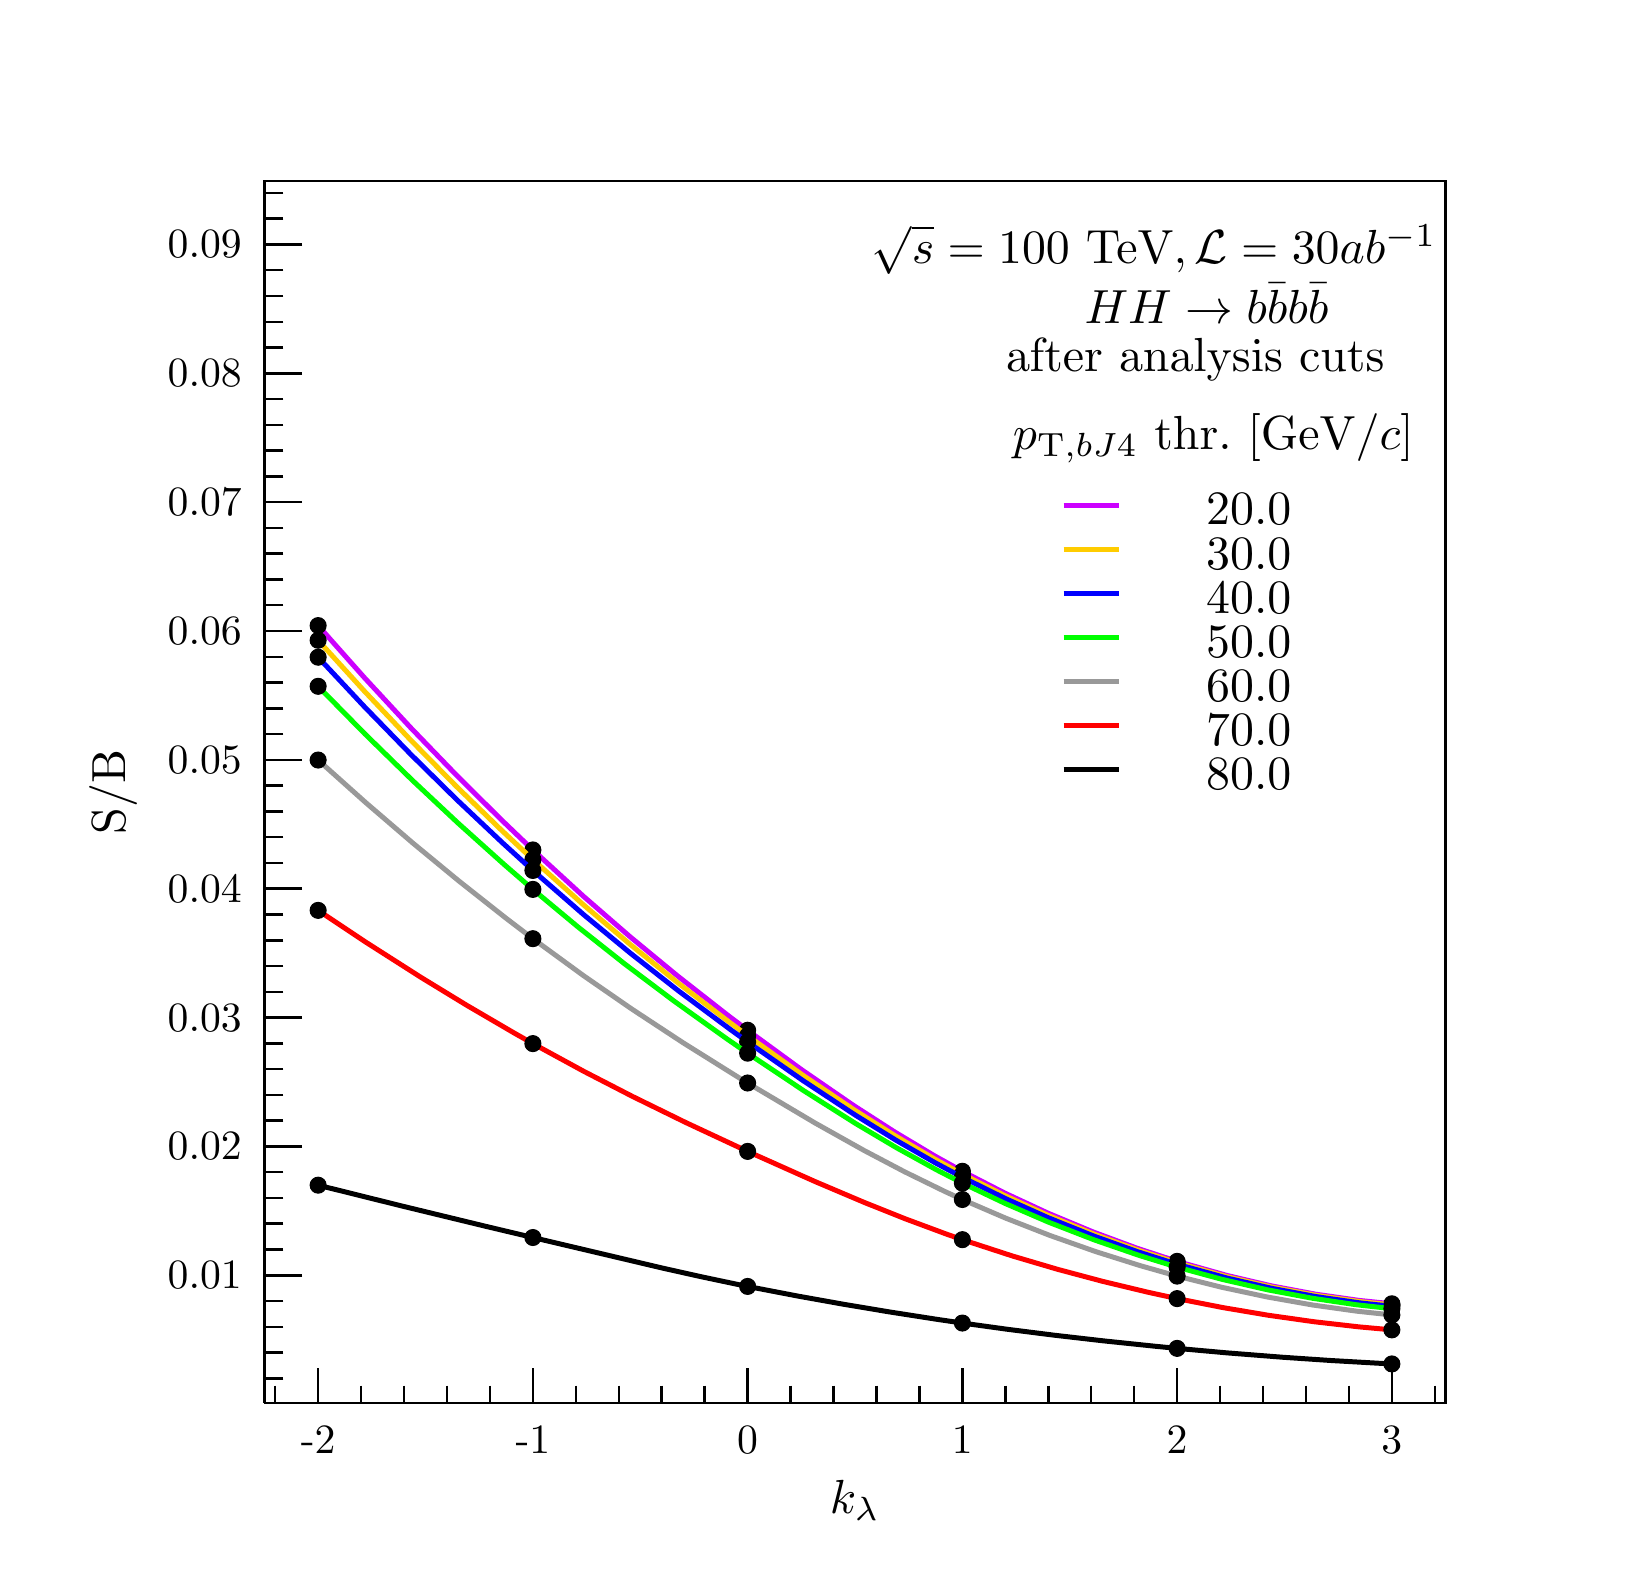
\begin{tikzpicture}
\pgfdeclareplotmark{cross} {
\pgfpathmoveto{\pgfpoint{-0.3\pgfplotmarksize}{\pgfplotmarksize}}
\pgfpathlineto{\pgfpoint{+0.3\pgfplotmarksize}{\pgfplotmarksize}}
\pgfpathlineto{\pgfpoint{+0.3\pgfplotmarksize}{0.3\pgfplotmarksize}}
\pgfpathlineto{\pgfpoint{+1\pgfplotmarksize}{0.3\pgfplotmarksize}}
\pgfpathlineto{\pgfpoint{+1\pgfplotmarksize}{-0.3\pgfplotmarksize}}
\pgfpathlineto{\pgfpoint{+0.3\pgfplotmarksize}{-0.3\pgfplotmarksize}}
\pgfpathlineto{\pgfpoint{+0.3\pgfplotmarksize}{-1.\pgfplotmarksize}}
\pgfpathlineto{\pgfpoint{-0.3\pgfplotmarksize}{-1.\pgfplotmarksize}}
\pgfpathlineto{\pgfpoint{-0.3\pgfplotmarksize}{-0.3\pgfplotmarksize}}
\pgfpathlineto{\pgfpoint{-1.\pgfplotmarksize}{-0.3\pgfplotmarksize}}
\pgfpathlineto{\pgfpoint{-1.\pgfplotmarksize}{0.3\pgfplotmarksize}}
\pgfpathlineto{\pgfpoint{-0.3\pgfplotmarksize}{0.3\pgfplotmarksize}}
\pgfpathclose
\pgfusepathqstroke
}
\pgfdeclareplotmark{cross*} {
\pgfpathmoveto{\pgfpoint{-0.3\pgfplotmarksize}{\pgfplotmarksize}}
\pgfpathlineto{\pgfpoint{+0.3\pgfplotmarksize}{\pgfplotmarksize}}
\pgfpathlineto{\pgfpoint{+0.3\pgfplotmarksize}{0.3\pgfplotmarksize}}
\pgfpathlineto{\pgfpoint{+1\pgfplotmarksize}{0.3\pgfplotmarksize}}
\pgfpathlineto{\pgfpoint{+1\pgfplotmarksize}{-0.3\pgfplotmarksize}}
\pgfpathlineto{\pgfpoint{+0.3\pgfplotmarksize}{-0.3\pgfplotmarksize}}
\pgfpathlineto{\pgfpoint{+0.3\pgfplotmarksize}{-1.\pgfplotmarksize}}
\pgfpathlineto{\pgfpoint{-0.3\pgfplotmarksize}{-1.\pgfplotmarksize}}
\pgfpathlineto{\pgfpoint{-0.3\pgfplotmarksize}{-0.3\pgfplotmarksize}}
\pgfpathlineto{\pgfpoint{-1.\pgfplotmarksize}{-0.3\pgfplotmarksize}}
\pgfpathlineto{\pgfpoint{-1.\pgfplotmarksize}{0.3\pgfplotmarksize}}
\pgfpathlineto{\pgfpoint{-0.3\pgfplotmarksize}{0.3\pgfplotmarksize}}
\pgfpathclose
\pgfusepathqfillstroke
}
\pgfdeclareplotmark{newstar} {
\pgfpathmoveto{\pgfqpoint{0pt}{\pgfplotmarksize}}
\pgfpathlineto{\pgfqpointpolar{44}{0.5\pgfplotmarksize}}
\pgfpathlineto{\pgfqpointpolar{18}{\pgfplotmarksize}}
\pgfpathlineto{\pgfqpointpolar{-20}{0.5\pgfplotmarksize}}
\pgfpathlineto{\pgfqpointpolar{-54}{\pgfplotmarksize}}
\pgfpathlineto{\pgfqpointpolar{-90}{0.5\pgfplotmarksize}}
\pgfpathlineto{\pgfqpointpolar{234}{\pgfplotmarksize}}
\pgfpathlineto{\pgfqpointpolar{198}{0.5\pgfplotmarksize}}
\pgfpathlineto{\pgfqpointpolar{162}{\pgfplotmarksize}}
\pgfpathlineto{\pgfqpointpolar{134}{0.5\pgfplotmarksize}}
\pgfpathclose
\pgfusepathqstroke
}
\pgfdeclareplotmark{newstar*} {
\pgfpathmoveto{\pgfqpoint{0pt}{\pgfplotmarksize}}
\pgfpathlineto{\pgfqpointpolar{44}{0.5\pgfplotmarksize}}
\pgfpathlineto{\pgfqpointpolar{18}{\pgfplotmarksize}}
\pgfpathlineto{\pgfqpointpolar{-20}{0.5\pgfplotmarksize}}
\pgfpathlineto{\pgfqpointpolar{-54}{\pgfplotmarksize}}
\pgfpathlineto{\pgfqpointpolar{-90}{0.5\pgfplotmarksize}}
\pgfpathlineto{\pgfqpointpolar{234}{\pgfplotmarksize}}
\pgfpathlineto{\pgfqpointpolar{198}{0.5\pgfplotmarksize}}
\pgfpathlineto{\pgfqpointpolar{162}{\pgfplotmarksize}}
\pgfpathlineto{\pgfqpointpolar{134}{0.5\pgfplotmarksize}}
\pgfpathclose
\pgfusepathqfillstroke
}
\definecolor{c}{rgb}{1,1,1};
\draw [color=c, fill=c] (0,0) rectangle (20,19.397);
\draw [color=c, fill=c] (3,1.9397) rectangle (18,17.4573);
\definecolor{c}{rgb}{0,0,0};
\draw [c,line width=0.9] (3,1.9397) -- (3,17.4573) -- (18,17.4573) -- (18,1.9397) -- (3,1.9397);
\definecolor{c}{rgb}{1,1,1};
\draw [color=c, fill=c] (3,1.9397) rectangle (18,17.4573);
\definecolor{c}{rgb}{0,0,0};
\draw [c,line width=0.9] (3,1.9397) -- (3,17.4573) -- (18,17.4573) -- (18,1.9397) -- (3,1.9397);
\draw [c,line width=0.9] (3,1.9397) -- (18,1.9397);
\draw [c,line width=0.9] (3.68182,2.37613) -- (3.68182,1.9397);
\draw [c,line width=0.9] (4.22727,2.15791) -- (4.22727,1.9397);
\draw [c,line width=0.9] (4.77273,2.15791) -- (4.77273,1.9397);
\draw [c,line width=0.9] (5.31818,2.15791) -- (5.31818,1.9397);
\draw [c,line width=0.9] (5.86364,2.15791) -- (5.86364,1.9397);
\draw [c,line width=0.9] (6.40909,2.37613) -- (6.40909,1.9397);
\draw [c,line width=0.9] (6.95455,2.15791) -- (6.95455,1.9397);
\draw [c,line width=0.9] (7.5,2.15791) -- (7.5,1.9397);
\draw [c,line width=0.9] (8.04545,2.15791) -- (8.04545,1.9397);
\draw [c,line width=0.9] (8.59091,2.15791) -- (8.59091,1.9397);
\draw [c,line width=0.9] (9.13636,2.37613) -- (9.13636,1.9397);
\draw [c,line width=0.9] (9.68182,2.15791) -- (9.68182,1.9397);
\draw [c,line width=0.9] (10.2273,2.15791) -- (10.2273,1.9397);
\draw [c,line width=0.9] (10.7727,2.15791) -- (10.7727,1.9397);
\draw [c,line width=0.9] (11.3182,2.15791) -- (11.3182,1.9397);
\draw [c,line width=0.9] (11.8636,2.37613) -- (11.8636,1.9397);
\draw [c,line width=0.9] (12.4091,2.15791) -- (12.4091,1.9397);
\draw [c,line width=0.9] (12.9545,2.15791) -- (12.9545,1.9397);
\draw [c,line width=0.9] (13.5,2.15791) -- (13.5,1.9397);
\draw [c,line width=0.9] (14.0455,2.15791) -- (14.0455,1.9397);
\draw [c,line width=0.9] (14.5909,2.37613) -- (14.5909,1.9397);
\draw [c,line width=0.9] (15.1364,2.15791) -- (15.1364,1.9397);
\draw [c,line width=0.9] (15.6818,2.15791) -- (15.6818,1.9397);
\draw [c,line width=0.9] (16.2273,2.15791) -- (16.2273,1.9397);
\draw [c,line width=0.9] (16.7727,2.15791) -- (16.7727,1.9397);
\draw [c,line width=0.9] (17.3182,2.37613) -- (17.3182,1.9397);
\draw [c,line width=0.9] (3.68182,2.37613) -- (3.68182,1.9397);
\draw [c,line width=0.9] (3.13636,2.15791) -- (3.13636,1.9397);
\draw [c,line width=0.9] (17.3182,2.37613) -- (17.3182,1.9397);
\draw [c,line width=0.9] (17.8636,2.15791) -- (17.8636,1.9397);
\draw [anchor=base] (3.68182,1.2996) node[scale=1.50669, color=c, rotate=0]{-2};
\draw [anchor=base] (6.40909,1.2996) node[scale=1.50669, color=c, rotate=0]{-1};
\draw [anchor=base] (9.13636,1.2996) node[scale=1.50669, color=c, rotate=0]{0};
\draw [anchor=base] (11.8636,1.2996) node[scale=1.50669, color=c, rotate=0]{1};
\draw [anchor=base] (14.5909,1.2996) node[scale=1.50669, color=c, rotate=0]{2};
\draw [anchor=base] (17.3182,1.2996) node[scale=1.50669, color=c, rotate=0]{3};
\draw (10.5,0.698292) node[scale=1.7299, color=c, rotate=0]{$k_{\lambda}$};
\draw [c,line width=0.9] (3,1.9397) -- (3,17.4573);
\draw [c,line width=0.9] (3.48,3.55945) -- (3,3.55945);
\draw [c,line width=0.9] (3.24,3.88673) -- (3,3.88673);
\draw [c,line width=0.9] (3.24,4.214) -- (3,4.214);
\draw [c,line width=0.9] (3.24,4.54128) -- (3,4.54128);
\draw [c,line width=0.9] (3.24,4.86856) -- (3,4.86856);
\draw [c,line width=0.9] (3.48,5.19584) -- (3,5.19584);
\draw [c,line width=0.9] (3.24,5.52312) -- (3,5.52312);
\draw [c,line width=0.9] (3.24,5.8504) -- (3,5.8504);
\draw [c,line width=0.9] (3.24,6.17767) -- (3,6.17767);
\draw [c,line width=0.9] (3.24,6.50495) -- (3,6.50495);
\draw [c,line width=0.9] (3.48,6.83223) -- (3,6.83223);
\draw [c,line width=0.9] (3.24,7.15951) -- (3,7.15951);
\draw [c,line width=0.9] (3.24,7.48679) -- (3,7.48679);
\draw [c,line width=0.9] (3.24,7.81406) -- (3,7.81406);
\draw [c,line width=0.9] (3.24,8.14134) -- (3,8.14134);
\draw [c,line width=0.9] (3.48,8.46862) -- (3,8.46862);
\draw [c,line width=0.9] (3.24,8.7959) -- (3,8.7959);
\draw [c,line width=0.9] (3.24,9.12318) -- (3,9.12318);
\draw [c,line width=0.9] (3.24,9.45046) -- (3,9.45046);
\draw [c,line width=0.9] (3.24,9.77773) -- (3,9.77773);
\draw [c,line width=0.9] (3.48,10.105) -- (3,10.105);
\draw [c,line width=0.9] (3.24,10.4323) -- (3,10.4323);
\draw [c,line width=0.9] (3.24,10.7596) -- (3,10.7596);
\draw [c,line width=0.9] (3.24,11.0868) -- (3,11.0868);
\draw [c,line width=0.9] (3.24,11.4141) -- (3,11.4141);
\draw [c,line width=0.9] (3.48,11.7414) -- (3,11.7414);
\draw [c,line width=0.9] (3.24,12.0687) -- (3,12.0687);
\draw [c,line width=0.9] (3.24,12.396) -- (3,12.396);
\draw [c,line width=0.9] (3.24,12.7232) -- (3,12.7232);
\draw [c,line width=0.9] (3.24,13.0505) -- (3,13.0505);
\draw [c,line width=0.9] (3.48,13.3778) -- (3,13.3778);
\draw [c,line width=0.9] (3.24,13.7051) -- (3,13.7051);
\draw [c,line width=0.9] (3.24,14.0323) -- (3,14.0323);
\draw [c,line width=0.9] (3.24,14.3596) -- (3,14.3596);
\draw [c,line width=0.9] (3.24,14.6869) -- (3,14.6869);
\draw [c,line width=0.9] (3.48,15.0142) -- (3,15.0142);
\draw [c,line width=0.9] (3.24,15.3415) -- (3,15.3415);
\draw [c,line width=0.9] (3.24,15.6687) -- (3,15.6687);
\draw [c,line width=0.9] (3.24,15.996) -- (3,15.996);
\draw [c,line width=0.9] (3.24,16.3233) -- (3,16.3233);
\draw [c,line width=0.9] (3.48,16.6506) -- (3,16.6506);
\draw [c,line width=0.9] (3.48,3.55945) -- (3,3.55945);
\draw [c,line width=0.9] (3.24,3.23217) -- (3,3.23217);
\draw [c,line width=0.9] (3.24,2.90489) -- (3,2.90489);
\draw [c,line width=0.9] (3.24,2.57761) -- (3,2.57761);
\draw [c,line width=0.9] (3.24,2.25034) -- (3,2.25034);
\draw [c,line width=0.9] (3.48,16.6506) -- (3,16.6506);
\draw [c,line width=0.9] (3.24,16.9779) -- (3,16.9779);
\draw [c,line width=0.9] (3.24,17.3051) -- (3,17.3051);
\draw [anchor= east] (2.9,3.55945) node[scale=1.50669, color=c, rotate=0]{0.01};
\draw [anchor= east] (2.9,5.19584) node[scale=1.50669, color=c, rotate=0]{0.02};
\draw [anchor= east] (2.9,6.83223) node[scale=1.50669, color=c, rotate=0]{0.03};
\draw [anchor= east] (2.9,8.46862) node[scale=1.50669, color=c, rotate=0]{0.04};
\draw [anchor= east] (2.9,10.105) node[scale=1.50669, color=c, rotate=0]{0.05};
\draw [anchor= east] (2.9,11.7414) node[scale=1.50669, color=c, rotate=0]{0.06};
\draw [anchor= east] (2.9,13.3778) node[scale=1.50669, color=c, rotate=0]{0.07};
\draw [anchor= east] (2.9,15.0142) node[scale=1.50669, color=c, rotate=0]{0.08};
\draw [anchor= east] (2.9,16.6506) node[scale=1.50669, color=c, rotate=0]{0.09};
\draw (1.08,9.69849) node[scale=1.7299, color=c, rotate=90]{S/B};
\definecolor{c}{rgb}{0.8,0,1};
\draw [c,line width=1.8] (3.68182,11.8104) -- (4.26766,11.151) -- (4.85584,10.515) -- (5.43415,9.91513) -- (6.00963,9.34322) -- (6.40909,8.96089) -- (7.05051,8.37335) -- (7.64181,7.86003) -- (8.24406,7.36317) -- (8.88688,6.85957) -- (9.13636,6.67108)
 -- (9.81911,6.17243) -- (10.4824,5.7156) -- (11.0032,5.38025) -- (11.5078,5.07805) -- (11.8636,4.88002) -- (12.4031,4.60312) -- (12.951,4.34846) -- (13.5304,4.10718) -- (14.0814,3.90337) -- (14.5909,3.73622) -- (15.2284,3.5561) -- (15.7944,3.42384)
 -- (16.3546,3.31858) -- (16.9052,3.23996) -- (17.3182,3.19716);
\definecolor{c}{rgb}{0,0,0};
\foreach \P in {(3.68182,11.8104), (6.40909,8.96089), (9.13636,6.67108), (11.8636,4.88002), (14.5909,3.73622), (17.3182,3.19716)}{\draw[mark options={color=c,fill=c},mark size=2.882883pt,mark=*] plot coordinates {\P};}
\definecolor{c}{rgb}{1,0.8,0};
\draw [c,line width=1.8] (3.68182,11.6239) -- (4.26816,10.9788) -- (4.85679,10.3568) -- (5.43527,9.7704) -- (6.0114,9.2109) -- (6.40909,8.83894) -- (7.05087,8.26467) -- (7.64314,7.76261) -- (8.25146,7.2726) -- (8.90558,6.77213) -- (9.13636,6.60159)
 -- (9.83149,6.10421) -- (10.4919,5.65815) -- (11.011,5.33005) -- (11.5145,5.03406) -- (11.8636,4.84324) -- (12.4025,4.57153) -- (12.9506,4.32119) -- (13.5311,4.08358) -- (14.0849,3.8821) -- (14.5909,3.71855) -- (15.2285,3.54058) -- (15.7963,3.40919)
 -- (16.3573,3.30442) -- (16.9102,3.22553) -- (17.3182,3.18283);
\definecolor{c}{rgb}{0,0,0};
\foreach \P in {(3.68182,11.6239), (6.40909,8.83894), (9.13636,6.60159), (11.8636,4.84324), (14.5909,3.71855), (17.3182,3.18283)}{\draw[mark options={color=c,fill=c},mark size=2.882883pt,mark=*] plot coordinates {\P};}
\definecolor{c}{rgb}{0,0,1};
\draw [c,line width=1.8] (3.68182,11.4085) -- (4.27093,10.7786) -- (4.86198,10.1715) -- (5.44146,9.60057) -- (6.02112,9.05342) -- (6.40909,8.70058) -- (7.05137,8.14155) -- (7.64645,7.65089) -- (8.26056,7.16967) -- (8.9244,6.67544) --
 (9.13636,6.52283) -- (9.84231,6.02995) -- (10.5006,5.59574) -- (11.0193,5.27531) -- (11.5239,4.98531) -- (11.8636,4.80361) -- (12.4041,4.53661) -- (12.9541,4.2904) -- (13.5351,4.057) -- (14.0919,3.858) -- (14.5909,3.69919) -- (15.2287,3.52328) --
 (15.7986,3.39252) -- (16.3606,3.28794) -- (16.9163,3.20836) -- (17.3182,3.16556);
\definecolor{c}{rgb}{0,0,0};
\foreach \P in {(3.68182,11.4085), (6.40909,8.70058), (9.13636,6.52283), (11.8636,4.80361), (14.5909,3.69919), (17.3182,3.16556)}{\draw[mark options={color=c,fill=c},mark size=2.882883pt,mark=*] plot coordinates {\P};}
\definecolor{c}{rgb}{0,1,0};
\draw [c,line width=1.8] (3.68182,11.0392) -- (4.27689,10.4338) -- (4.87317,9.85107) -- (5.45498,9.30554) -- (6.04228,8.77793) -- (6.40909,8.46014) -- (6.98228,7.98281) -- (7.58086,7.509) -- (8.20374,7.04041) -- (8.87292,6.562) -- (9.13636,6.38013)
 -- (9.85404,5.90028) -- (10.5103,5.48532) -- (11.0294,5.17767) -- (11.5365,4.89792) -- (11.8636,4.72979) -- (12.4065,4.4716) -- (12.9595,4.23306) -- (13.542,4.00727) -- (14.1046,3.81283) -- (14.5909,3.66266) -- (15.1611,3.50776) -- (15.7356,3.37555)
 -- (16.3092,3.2674) -- (16.8646,3.1854) -- (17.3182,3.13501);
\definecolor{c}{rgb}{0,0,0};
\foreach \P in {(3.68182,11.0392), (6.40909,8.46014), (9.13636,6.38013), (11.8636,4.72979), (14.5909,3.66266), (17.3182,3.13501)}{\draw[mark options={color=c,fill=c},mark size=2.882883pt,mark=*] plot coordinates {\P};}
\definecolor{c}{rgb}{0.6,0.6,0.6};
\draw [c,line width=1.8] (3.68182,10.1029) -- (4.28363,9.56473) -- (4.88585,9.04751) -- (5.47062,8.56565) -- (6.06653,8.09523) -- (6.40909,7.83423) -- (7.05405,7.36322) -- (7.66274,6.9423) -- (8.31211,6.51538) -- (9.02753,6.06759) --
 (9.13636,6.00127) -- (9.9936,5.49285) -- (10.6179,5.14315) -- (11.1279,4.87473) -- (11.6409,4.62372) -- (11.8636,4.52142) -- (12.4171,4.28355) -- (12.977,4.06459) -- (13.5571,3.85999) -- (14.1196,3.68246) -- (14.5909,3.549) -- (15.1625,3.40592) --
 (15.7381,3.28309) -- (16.3121,3.18184) -- (16.8692,3.10384) -- (17.3182,3.05551);
\definecolor{c}{rgb}{0,0,0};
\foreach \P in {(3.68182,10.1029), (6.40909,7.83423), (9.13636,6.00127), (11.8636,4.52142), (14.5909,3.549), (17.3182,3.05551)}{\draw[mark options={color=c,fill=c},mark size=2.882883pt,mark=*] plot coordinates {\P};}
\definecolor{c}{rgb}{1,0,0};
\draw [c,line width=1.8] (3.68182,8.19352) -- (4.2902,7.78809) -- (4.98705,7.3435) -- (5.56833,6.98878) -- (6.17796,6.63253) -- (6.40909,6.50168) -- (7.0559,6.14941) -- (7.67251,5.83163) -- (8.35164,5.49889) -- (9.13636,5.13259) -- (9.99649,4.74806)
 -- (10.6236,4.48217) -- (11.1381,4.27674) -- (11.6555,4.08445) -- (11.8636,4.01169) -- (12.5019,3.80358) -- (13.0707,3.63562) -- (13.6435,3.48252) -- (14.2253,3.34293) -- (14.5909,3.26315) -- (15.1719,3.14912) -- (15.7557,3.05059) --
 (16.3323,2.96909) -- (16.9012,2.90406) -- (17.3182,2.86609);
\definecolor{c}{rgb}{0,0,0};
\foreach \P in {(3.68182,8.19352), (6.40909,6.50168), (9.13636,5.13259), (11.8636,4.01169), (14.5909,3.26315), (17.3182,2.86609)}{\draw[mark options={color=c,fill=c},mark size=2.882883pt,mark=*] plot coordinates {\P};}
\draw [c,line width=1.8] (3.68182,4.7036) -- (4.7319,4.44255) -- (5.80388,4.1827) -- (6.40909,4.03897) -- (8.05868,3.64991) -- (8.53886,3.54263) -- (9.01029,3.44317) -- (9.13636,3.41778) -- (9.77547,3.29503) -- (10.3499,3.19218) -- (10.9314,3.09493)
 -- (11.5333,3.00115) -- (11.8636,2.95252) -- (12.4357,2.87351) -- (13.0328,2.7981) -- (13.654,2.72666) -- (14.3199,2.65726) -- (14.5909,2.63095) -- (15.2329,2.57331) -- (15.9334,2.51825) -- (16.5415,2.4771) -- (17.1833,2.44035) -- (17.3182,2.4335);
\foreach \P in {(3.68182,4.7036), (6.40909,4.03897), (9.13636,3.41778), (11.8636,2.95252), (14.5909,2.63095), (17.3182,2.4335)}{\draw[mark options={color=c,fill=c},mark size=2.882883pt,mark=*] plot coordinates {\P};}
\draw [anchor=north] (15.05,14.7137) node[scale=1.7299, color=c, rotate=0]{$p_{\text{T}, bJ4} \text{~thr.} ~[\text{GeV}/c]$};
\draw [anchor=base] (15.5,13.649) node[scale=1.7299, color=c, rotate=0]{ };
\draw [anchor=base] (15.5,13.0887) node[scale=1.7299, color=c, rotate=0]{20.0};
\definecolor{c}{rgb}{0.8,0,1};
\draw [c,line width=1.8] (13.15,13.3408) -- (13.85,13.3408);
\definecolor{c}{rgb}{0,0,0};
\draw [anchor=base] (15.5,12.5283) node[scale=1.7299, color=c, rotate=0]{30.0};
\definecolor{c}{rgb}{1,0.8,0};
\draw [c,line width=1.8] (13.15,12.7805) -- (13.85,12.7805);
\definecolor{c}{rgb}{0,0,0};
\draw [anchor=base] (15.5,11.9679) node[scale=1.7299, color=c, rotate=0]{40.0};
\definecolor{c}{rgb}{0,0,1};
\draw [c,line width=1.8] (13.15,12.2201) -- (13.85,12.2201);
\definecolor{c}{rgb}{0,0,0};
\draw [anchor=base] (15.5,11.4076) node[scale=1.7299, color=c, rotate=0]{50.0};
\definecolor{c}{rgb}{0,1,0};
\draw [c,line width=1.8] (13.15,11.6597) -- (13.85,11.6597);
\definecolor{c}{rgb}{0,0,0};
\draw [anchor=base] (15.5,10.8472) node[scale=1.7299, color=c, rotate=0]{60.0};
\definecolor{c}{rgb}{0.6,0.6,0.6};
\draw [c,line width=1.8] (13.15,11.0994) -- (13.85,11.0994);
\definecolor{c}{rgb}{0,0,0};
\draw [anchor=base] (15.5,10.2869) node[scale=1.7299, color=c, rotate=0]{70.0};
\definecolor{c}{rgb}{1,0,0};
\draw [c,line width=1.8] (13.15,10.539) -- (13.85,10.539);
\definecolor{c}{rgb}{0,0,0};
\draw [anchor=base] (15.5,9.72651) node[scale=1.7299, color=c, rotate=0]{80.0};
\draw [c,line width=1.8] (13.15,9.97867) -- (13.85,9.97867);
\draw [anchor= west] (10.5,16.5844) node[scale=1.7299, color=c, rotate=0]{$\sqrt{s} = 100 ~\text{TeV}, \mathcal{L} = 30 ab^{-1}$};
\draw [anchor= west] (13.2,15.9055) node[scale=1.7299, color=c, rotate=0]{$HH \rightarrow b\bar{b}b\bar{b}$};
\draw [anchor=base west] (12.2,15.0424) node[scale=1.7299, color=c, rotate=0]{after analysis cuts};
\end{tikzpicture}
% end document
\end{document}
